\documentclass[]{article}
\usepackage{fullpage}
\usepackage{lastpage}
\usepackage[top=1in,bottom=1in,margin=1in]{geometry}
\usepackage{supertabular}
\usepackage{graphicx,tikz}	
%\usepackage{tkz-euclide}
%\usetkzobj{all}
\usetikzlibrary{calc}
\usepackage{array,multicol}
\usepackage{amsmath,amssymb}
\usepackage{enumitem}

\usepackage{fancyhdr}
\pagestyle{fancy}

\addtolength{\topmargin}{-0.25in}

\newcommand{\vect}[1]{\mathbf{#1}}
\DeclareMathOperator{\proj}{proj}

\fancypagestyle{plain}{
	\addtolength{\headheight}{0.485in}
	\rhead{\bf MATH 2574 (Calculus III) \\
		%\vspace{0.5pc}
		Wed 1 Mar 2017 \\}
	\rfoot{\footnotesize $\;$Quiz 5IC, p. \thepage\ (of \pageref{LastPage})
	}
\renewcommand{\headrulewidth}{0pt}
}
\fancyhf{}
\renewcommand{\headrulewidth}{0pt}
\rfoot{\footnotesize Quiz 5IC, p. \thepage\ (of \pageref{LastPage})$\;$}

\title{\vspace{-3.5pc} 
	\flushleft \bf \Large In-Class Quiz 5: Polar coordinates \\ (\S 10.1-10.3)}
\date{}

% % % % %
\begin{document}
\maketitle

\vspace{-3pc}
\noindent{\bf Directions:} This quiz is due at the end of lecture.  

\noindent\hrulefill

\begin{enumerate}

% % %
\item %{\bf \S10.2 \#52}
The figure on the left is a Cartesian graph of the polar function 
\[
r=\cos{\theta}+\sin{2\theta}.
\]
The polar graph is on the right.  Mark the points on the polar graph that correspond to the points shown on the Cartesian graph.

\begin{center}
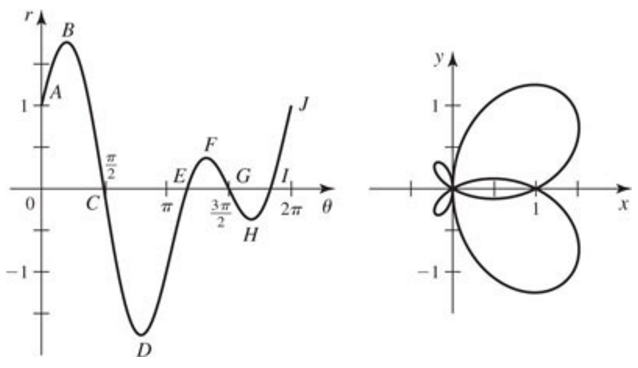
\includegraphics[scale=1.1]{Q5pic}
\end{center}

\newpage
% % %
\item %{\bf \S10.3}
The area of the region bounded by a polar graph $r=f(\theta)$ between the angles $\alpha$ and $\beta$ is given by the formula
\[
\frac{1}{2}\int_{\alpha}^{\beta}f(\theta)^2\ d\theta.
\]
Graph the rose $r=2\cos{3\theta}$ and then find its area. 

% % % % %
\end{enumerate}
\end{document}